\documentclass[fleqn,amsmath,amssymb,superscriptaddress, reprint,prl]{revtex4-1}
\usepackage{graphicx} %include figure files
\usepackage{dcolumn} %align table columns on decimal point (?)
\usepackage{bm} %bold math
\usepackage{hyperref} %add hypertext capabilities
\usepackage{longtable} % for tables with figures
\usepackage[T1]{fontenc}
\usepackage{times}
\usepackage{lipsum}
\usepackage{xcolor}
\usepackage{enumitem}
\usepackage{outlines}
\graphicspath{{figures/} }
\renewcommand{\UrlFont}{\small}
\newcommand\red[1]{\textcolor{red}{#1}}
\newcommand\blue[1]{\textcolor{blue}{#1}}
\newcommand\purple[1]{\textcolor{purple}{#1}}
\newcommand{\eg} {\textit{e.g.} }
\newcommand{\ie} {\textit{i.e.} }
\renewcommand{\figurename} {Figure}
\renewcommand{\thefigure} {\arabic{figure}}
\maxdeadcycles=200
\begin{document}


\begin{figure}
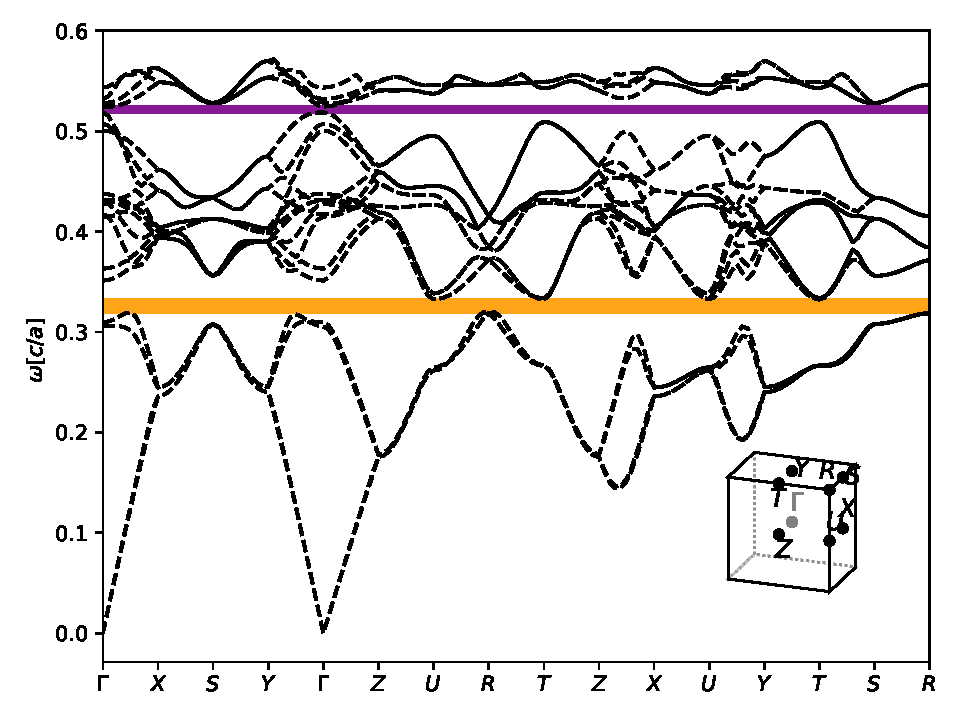
\includegraphics[width=0.9\linewidth]{workspace/1563e583794690e0dd79d3b6d35d7618/images/r=15.pdf}
	\caption{\textbf{Pyrochlore- Related Cesium Tellurium Oxide ($oP$44-Te\textsubscript{4}CO\textsubscript{6}) at $\phi=0.37$}. (1) 3.6\% gap between bands 4-5, and (2) 1.49\% gap between bands 16-17.}
\end{figure}

\begin{figure}
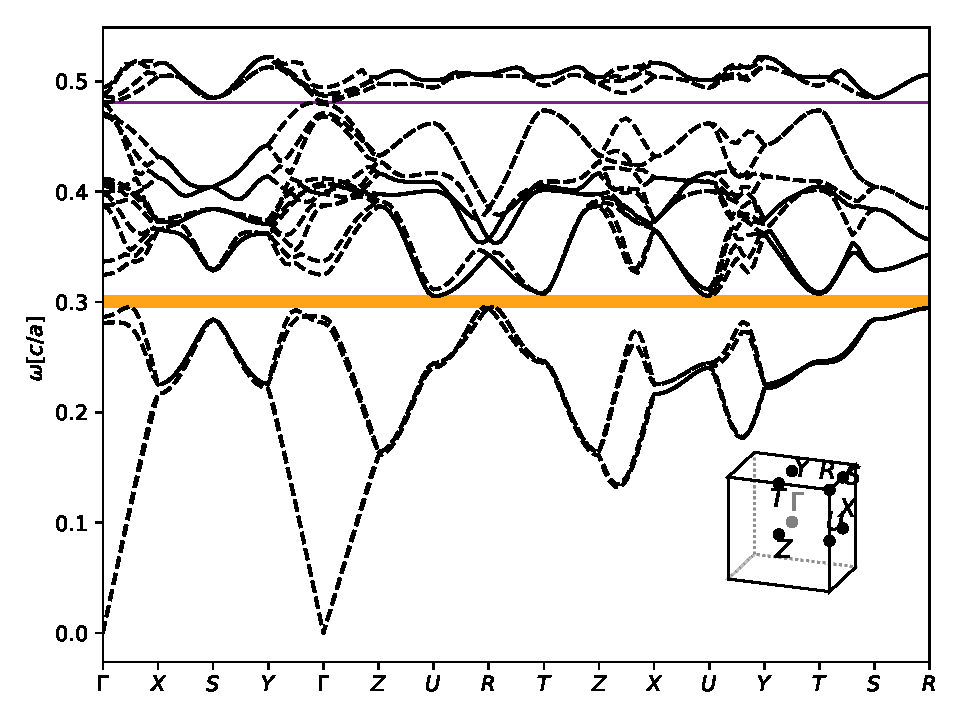
\includegraphics[width=0.9\linewidth]{workspace/1563e583794690e0dd79d3b6d35d7618/images/r=16.pdf}
	\caption{\textbf{Pyrochlore- Related Cesium Tellurium Oxide ($oP$44-Te\textsubscript{4}CO\textsubscript{6}) at $\phi=0.43$}. (1) 4.27\% gap between bands 4-5, and (2) 1.15\% gap between bands 16-17.}
\end{figure}
\end{document}